\documentclass[twoside]{book}

% Packages required by doxygen
\usepackage{calc}
\usepackage{doxygen}
\usepackage{graphicx}
\usepackage[utf8]{inputenc}
\usepackage{makeidx}
\usepackage{multicol}
\usepackage{multirow}
\usepackage{textcomp}
\usepackage[table]{xcolor}

% Font selection
\usepackage[T1]{fontenc}
\usepackage{mathptmx}
\usepackage[scaled=.90]{helvet}
\usepackage{courier}
\usepackage{amssymb}
\usepackage{sectsty}
\renewcommand{\familydefault}{\sfdefault}
\allsectionsfont{%
  \fontseries{bc}\selectfont%
  \color{darkgray}%
}
\renewcommand{\DoxyLabelFont}{%
  \fontseries{bc}\selectfont%
  \color{darkgray}%
}

% Page & text layout
\usepackage{geometry}
\geometry{%
  a4paper,%
  top=2.5cm,%
  bottom=2.5cm,%
  left=2.5cm,%
  right=2.5cm%
}
\tolerance=750
\hfuzz=15pt
\hbadness=750
\setlength{\emergencystretch}{15pt}
\setlength{\parindent}{0cm}
\setlength{\parskip}{0.2cm}
\makeatletter
\renewcommand{\paragraph}{%
  \@startsection{paragraph}{4}{0ex}{-1.0ex}{1.0ex}{%
    \normalfont\normalsize\bfseries\SS@parafont%
  }%
}
\renewcommand{\subparagraph}{%
  \@startsection{subparagraph}{5}{0ex}{-1.0ex}{1.0ex}{%
    \normalfont\normalsize\bfseries\SS@subparafont%
  }%
}
\makeatother

% Headers & footers
\usepackage{fancyhdr}
\pagestyle{fancyplain}
\fancyhead[LE]{\fancyplain{}{\bfseries\thepage}}
\fancyhead[CE]{\fancyplain{}{}}
\fancyhead[RE]{\fancyplain{}{\bfseries\leftmark}}
\fancyhead[LO]{\fancyplain{}{\bfseries\rightmark}}
\fancyhead[CO]{\fancyplain{}{}}
\fancyhead[RO]{\fancyplain{}{\bfseries\thepage}}
\fancyfoot[LE]{\fancyplain{}{}}
\fancyfoot[CE]{\fancyplain{}{}}
\fancyfoot[RE]{\fancyplain{}{\bfseries\scriptsize Generated on Wed Mar 18 2015 22\-:39\-:07 for S\-F\-X by Doxygen }}
\fancyfoot[LO]{\fancyplain{}{\bfseries\scriptsize Generated on Wed Mar 18 2015 22\-:39\-:07 for S\-F\-X by Doxygen }}
\fancyfoot[CO]{\fancyplain{}{}}
\fancyfoot[RO]{\fancyplain{}{}}
\renewcommand{\footrulewidth}{0.4pt}
\renewcommand{\chaptermark}[1]{%
  \markboth{#1}{}%
}
\renewcommand{\sectionmark}[1]{%
  \markright{\thesection\ #1}%
}

% Indices & bibliography
\usepackage{natbib}
\usepackage[titles]{tocloft}
\setcounter{tocdepth}{3}
\setcounter{secnumdepth}{5}
\makeindex

% Hyperlinks (required, but should be loaded last)
\usepackage{ifpdf}
\ifpdf
  \usepackage[pdftex,pagebackref=true]{hyperref}
\else
  \usepackage[ps2pdf,pagebackref=true]{hyperref}
\fi
\hypersetup{%
  colorlinks=true,%
  linkcolor=blue,%
  citecolor=blue,%
  unicode%
}

% Custom commands
\newcommand{\clearemptydoublepage}{%
  \newpage{\pagestyle{empty}\cleardoublepage}%
}


%===== C O N T E N T S =====

\begin{document}

% Titlepage & ToC
\hypersetup{pageanchor=false}
\pagenumbering{roman}
\begin{titlepage}
\vspace*{7cm}
\begin{center}%
{\Large S\-F\-X }\\
\vspace*{1cm}
{\large Generated by Doxygen 1.8.5}\\
\vspace*{0.5cm}
{\small Wed Mar 18 2015 22:39:07}\\
\end{center}
\end{titlepage}
\clearemptydoublepage
\tableofcontents
\clearemptydoublepage
\pagenumbering{arabic}
\hypersetup{pageanchor=true}

%--- Begin generated contents ---
\chapter{Hierarchical Index}
\section{Class Hierarchy}
This inheritance list is sorted roughly, but not completely, alphabetically\-:\begin{DoxyCompactList}
\item \contentsline{section}{model}{\pageref{classmodel}}{}
\item \contentsline{section}{Utility}{\pageref{class_utility}}{}
\item wx\-App\begin{DoxyCompactList}
\item \contentsline{section}{sfx\-App}{\pageref{classsfx_app}}{}
\end{DoxyCompactList}
\item wx\-Dialog\begin{DoxyCompactList}
\item \contentsline{section}{Detail\-Dialog}{\pageref{class_detail_dialog}}{}
\end{DoxyCompactList}
\item wx\-Frame\begin{DoxyCompactList}
\item \contentsline{section}{sfx\-Frame}{\pageref{classsfx_frame}}{}
\end{DoxyCompactList}
\end{DoxyCompactList}

\chapter{Class Index}
\section{Class List}
Here are the classes, structs, unions and interfaces with brief descriptions\-:\begin{DoxyCompactList}
\item\contentsline{section}{\hyperlink{class_detail_dialog}{Detail\-Dialog} }{\pageref{class_detail_dialog}}{}
\item\contentsline{section}{\hyperlink{classmodel}{model} }{\pageref{classmodel}}{}
\item\contentsline{section}{\hyperlink{classsfx_app}{sfx\-App} \\*Defines Application Class. Machine generated }{\pageref{classsfx_app}}{}
\item\contentsline{section}{\hyperlink{classsfx_frame}{sfx\-Frame} }{\pageref{classsfx_frame}}{}
\item\contentsline{section}{\hyperlink{class_utility}{Utility} }{\pageref{class_utility}}{}
\end{DoxyCompactList}

\chapter{Class Documentation}
\hypertarget{class_detail_dialog}{\section{Detail\-Dialog Class Reference}
\label{class_detail_dialog}\index{Detail\-Dialog@{Detail\-Dialog}}
}
Inheritance diagram for Detail\-Dialog\-:\begin{figure}[H]
\begin{center}
\leavevmode
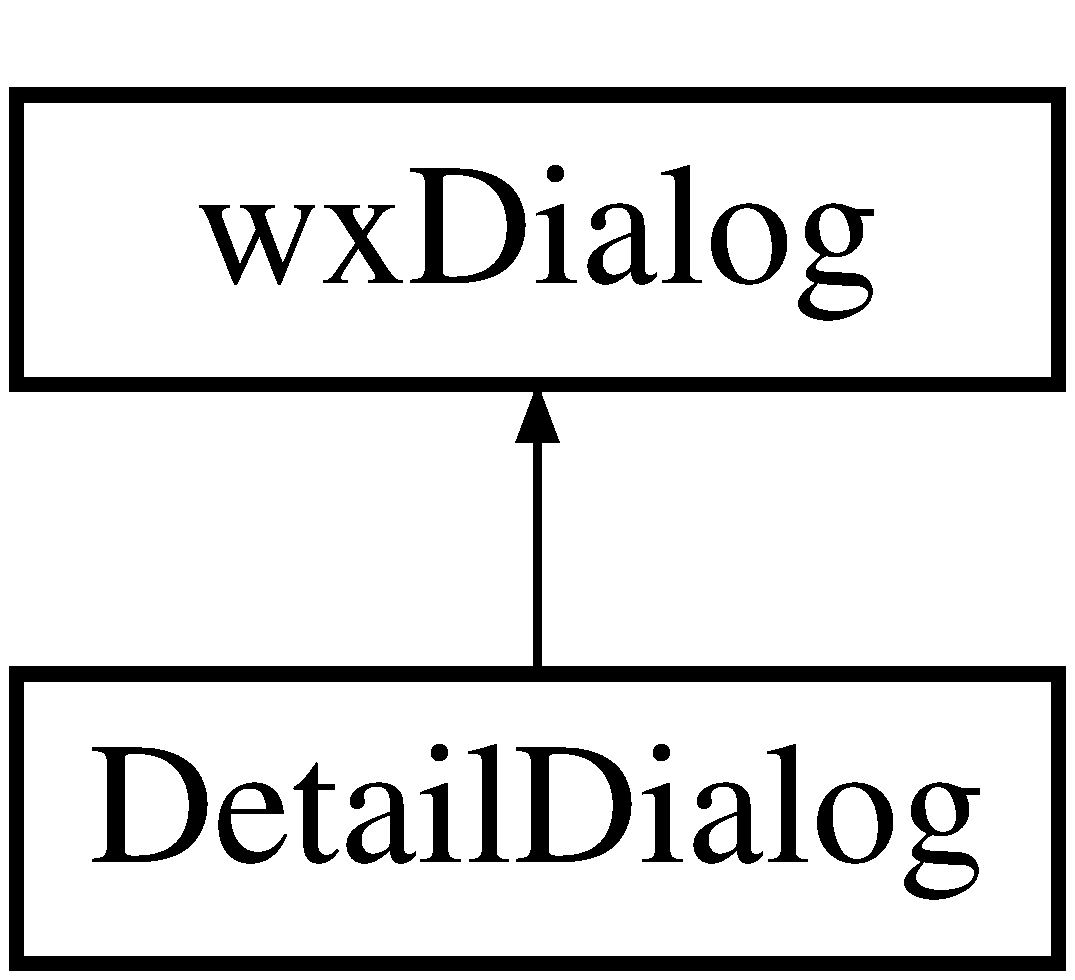
\includegraphics[height=2.000000cm]{class_detail_dialog}
\end{center}
\end{figure}
\subsection*{Public Member Functions}
\begin{DoxyCompactItemize}
\item 
\hyperlink{class_detail_dialog_afd8f2713c0edd1b672227cda0f6b9d54}{Detail\-Dialog} (wx\-Window $\ast$parent, wx\-String filename, wx\-String description, wx\-Window\-I\-D id=wx\-I\-D\-\_\-\-A\-N\-Y, const wx\-Point \&pos=wx\-Default\-Position)
\begin{DoxyCompactList}\small\item\em Constructor. \end{DoxyCompactList}\item 
virtual \hyperlink{class_detail_dialog_abbee914db783bd3207a1697e1f41eef2}{$\sim$\-Detail\-Dialog} ()
\end{DoxyCompactItemize}
\subsection*{Public Attributes}
\begin{DoxyCompactItemize}
\item 
\hypertarget{class_detail_dialog_abbe706e5374b5d84c9f5dfcee5712372}{wx\-Button $\ast$ {\bfseries Play\-Button}}\label{class_detail_dialog_abbe706e5374b5d84c9f5dfcee5712372}

\item 
\hypertarget{class_detail_dialog_a5d1e5dad94eeb3e768d4bd83a0d0fa58}{wx\-Static\-Text $\ast$ {\bfseries Description\-Static\-Text}}\label{class_detail_dialog_a5d1e5dad94eeb3e768d4bd83a0d0fa58}

\item 
\hypertarget{class_detail_dialog_a76a63ab17e950703a3c99e6ed36b1500}{wx\-Panel $\ast$ {\bfseries Panel1}}\label{class_detail_dialog_a76a63ab17e950703a3c99e6ed36b1500}

\item 
\hypertarget{class_detail_dialog_adfcb62c539f6f26f8e9f6674e08ac57e}{wx\-Static\-Text $\ast$ {\bfseries Static\-Text1}}\label{class_detail_dialog_adfcb62c539f6f26f8e9f6674e08ac57e}

\item 
\hypertarget{class_detail_dialog_ab8957eb1fd159c1e50c945b0ed99295c}{wx\-Button $\ast$ {\bfseries Exit\-Button}}\label{class_detail_dialog_ab8957eb1fd159c1e50c945b0ed99295c}

\item 
\hypertarget{class_detail_dialog_ad3a9ba29c509e8fdb9adf05df691cfb2}{wx\-Static\-Text $\ast$ {\bfseries Static\-Text3}}\label{class_detail_dialog_ad3a9ba29c509e8fdb9adf05df691cfb2}

\item 
\hypertarget{class_detail_dialog_ab63cadc52242ec0de074174a093be884}{wx\-Static\-Box $\ast$ {\bfseries Static\-Box1}}\label{class_detail_dialog_ab63cadc52242ec0de074174a093be884}

\item 
\hypertarget{class_detail_dialog_af5251d3b55705d40bed2e6204dae18a1}{wx\-Static\-Text $\ast$ {\bfseries Channels\-Static\-Text}}\label{class_detail_dialog_af5251d3b55705d40bed2e6204dae18a1}

\item 
\hypertarget{class_detail_dialog_a411a248198f8c1f5933e43126f7aba95}{wx\-Button $\ast$ {\bfseries Stop\-Button}}\label{class_detail_dialog_a411a248198f8c1f5933e43126f7aba95}

\item 
\hypertarget{class_detail_dialog_aa7af7eb32d948c195e51077f61b65d4c}{wx\-Static\-Text $\ast$ {\bfseries Samplerate\-Static\-Text}}\label{class_detail_dialog_aa7af7eb32d948c195e51077f61b65d4c}

\item 
\hypertarget{class_detail_dialog_aacb52a65130dc95e51d43fc144a679dd}{wx\-Static\-Text $\ast$ {\bfseries Static\-Text4}}\label{class_detail_dialog_aacb52a65130dc95e51d43fc144a679dd}

\end{DoxyCompactItemize}
\subsection*{Static Protected Attributes}
\begin{DoxyCompactItemize}
\item 
static const long \hyperlink{class_detail_dialog_abed1d78f4aa5a1f0d57364604462adb3}{I\-D\-\_\-\-S\-T\-A\-T\-I\-C\-B\-O\-X1} = wx\-New\-Id()
\item 
\hypertarget{class_detail_dialog_a8e723de7467321b855d6a9d113df4e55}{static const long {\bfseries I\-D\-\_\-\-S\-T\-A\-T\-I\-C\-T\-E\-X\-T3} = wx\-New\-Id()}\label{class_detail_dialog_a8e723de7467321b855d6a9d113df4e55}

\item 
\hypertarget{class_detail_dialog_a0772eec8444ca8ed510afe21a0c12342}{static const long {\bfseries I\-D\-\_\-\-S\-T\-A\-T\-I\-C\-T\-E\-X\-T4} = wx\-New\-Id()}\label{class_detail_dialog_a0772eec8444ca8ed510afe21a0c12342}

\item 
\hypertarget{class_detail_dialog_a35b8def37c9fcb69bd3bacbab15803e6}{static const long {\bfseries I\-D\-\_\-\-S\-T\-A\-T\-I\-C\-T\-E\-X\-T1} = wx\-New\-Id()}\label{class_detail_dialog_a35b8def37c9fcb69bd3bacbab15803e6}

\item 
\hypertarget{class_detail_dialog_a0cd6d945f5f7e3a128fda2461c8472cc}{static const long {\bfseries I\-D\-\_\-\-S\-T\-A\-T\-I\-C\-T\-E\-X\-T5} = wx\-New\-Id()}\label{class_detail_dialog_a0cd6d945f5f7e3a128fda2461c8472cc}

\item 
\hypertarget{class_detail_dialog_af55176f0dac7fcf7cab91a05086016e9}{static const long {\bfseries I\-D\-\_\-\-P\-A\-N\-E\-L1} = wx\-New\-Id()}\label{class_detail_dialog_af55176f0dac7fcf7cab91a05086016e9}

\item 
\hypertarget{class_detail_dialog_a62761535becea9e8e833683702c28f3d}{static const long {\bfseries I\-D\-\_\-\-B\-U\-T\-T\-O\-N1} = wx\-New\-Id()}\label{class_detail_dialog_a62761535becea9e8e833683702c28f3d}

\item 
\hypertarget{class_detail_dialog_adeb0db3c34824232f3f2c5554b068180}{static const long {\bfseries I\-D\-\_\-\-B\-U\-T\-T\-O\-N2} = wx\-New\-Id()}\label{class_detail_dialog_adeb0db3c34824232f3f2c5554b068180}

\item 
\hypertarget{class_detail_dialog_afda7240a12907c289f3fa2166edb4398}{static const long {\bfseries I\-D\-\_\-\-B\-U\-T\-T\-O\-N3} = wx\-New\-Id()}\label{class_detail_dialog_afda7240a12907c289f3fa2166edb4398}

\item 
\hypertarget{class_detail_dialog_a20a72303e5db79e02106aaa10acdb5d4}{static const long {\bfseries I\-D\-\_\-\-S\-T\-A\-T\-I\-C\-T\-E\-X\-T7} = wx\-New\-Id()}\label{class_detail_dialog_a20a72303e5db79e02106aaa10acdb5d4}

\item 
\hypertarget{class_detail_dialog_addf7ae0faaa160502540bfc29749a2c7}{static const long {\bfseries I\-D\-\_\-\-S\-T\-A\-T\-I\-C\-T\-E\-X\-T8} = wx\-New\-Id()}\label{class_detail_dialog_addf7ae0faaa160502540bfc29749a2c7}

\end{DoxyCompactItemize}


\subsection{Detailed Description}


Definition at line 28 of file Detail\-Dialog.\-h.



\subsection{Constructor \& Destructor Documentation}
\hypertarget{class_detail_dialog_afd8f2713c0edd1b672227cda0f6b9d54}{\index{Detail\-Dialog@{Detail\-Dialog}!Detail\-Dialog@{Detail\-Dialog}}
\index{Detail\-Dialog@{Detail\-Dialog}!DetailDialog@{Detail\-Dialog}}
\subsubsection[{Detail\-Dialog}]{\setlength{\rightskip}{0pt plus 5cm}Detail\-Dialog\-::\-Detail\-Dialog (
\begin{DoxyParamCaption}
\item[{wx\-Window $\ast$}]{parent, }
\item[{wx\-String}]{filename, }
\item[{wx\-String}]{description, }
\item[{wx\-Window\-I\-D}]{id = {\ttfamily wxID\-\_\-ANY}, }
\item[{const wx\-Point \&}]{pos = {\ttfamily wxDefaultPosition}}
\end{DoxyParamCaption}
)}}\label{class_detail_dialog_afd8f2713c0edd1b672227cda0f6b9d54}


Constructor. 

Machine generated event table.
\begin{DoxyParams}{Parameters}
{\em parent} & Parent window (S\-F\-X main window). \\
\hline
{\em filename} & Full path to filename to load. \\
\hline
{\em description} & Description of this sound effect as loaded from datafile. \\
\hline
{\em id} & Machine genereated window I\-D; gets value as def arg. \\
\hline
{\em pos} & Machine generated position; gets value as def arg. \\
\hline
\end{DoxyParams}
Create buffers in which we will draw the waveform and its inverse.

Show description of this sound effect.

Set up a path for the temp files.

Load the W\-A\-V file that was passed to this dialog.

Show info we read from the W\-A\-V file.

Remember description to use as a prefix for the W\-A\-V filename we generate. 

Definition at line 81 of file Detail\-Dialog.\-cpp.

\hypertarget{class_detail_dialog_abbee914db783bd3207a1697e1f41eef2}{\index{Detail\-Dialog@{Detail\-Dialog}!$\sim$\-Detail\-Dialog@{$\sim$\-Detail\-Dialog}}
\index{$\sim$\-Detail\-Dialog@{$\sim$\-Detail\-Dialog}!DetailDialog@{Detail\-Dialog}}
\subsubsection[{$\sim$\-Detail\-Dialog}]{\setlength{\rightskip}{0pt plus 5cm}Detail\-Dialog\-::$\sim$\-Detail\-Dialog (
\begin{DoxyParamCaption}
{}
\end{DoxyParamCaption}
)\hspace{0.3cm}{\ttfamily [virtual]}}}\label{class_detail_dialog_abbee914db783bd3207a1697e1f41eef2}
Delete background buffers. 

Definition at line 162 of file Detail\-Dialog.\-cpp.



\subsection{Member Data Documentation}
\hypertarget{class_detail_dialog_abed1d78f4aa5a1f0d57364604462adb3}{\index{Detail\-Dialog@{Detail\-Dialog}!I\-D\-\_\-\-S\-T\-A\-T\-I\-C\-B\-O\-X1@{I\-D\-\_\-\-S\-T\-A\-T\-I\-C\-B\-O\-X1}}
\index{I\-D\-\_\-\-S\-T\-A\-T\-I\-C\-B\-O\-X1@{I\-D\-\_\-\-S\-T\-A\-T\-I\-C\-B\-O\-X1}!DetailDialog@{Detail\-Dialog}}
\subsubsection[{I\-D\-\_\-\-S\-T\-A\-T\-I\-C\-B\-O\-X1}]{\setlength{\rightskip}{0pt plus 5cm}const long Detail\-Dialog\-::\-I\-D\-\_\-\-S\-T\-A\-T\-I\-C\-B\-O\-X1 = wx\-New\-Id()\hspace{0.3cm}{\ttfamily [static]}, {\ttfamily [protected]}}}\label{class_detail_dialog_abed1d78f4aa5a1f0d57364604462adb3}
Constants. 

Definition at line 59 of file Detail\-Dialog.\-h.



The documentation for this class was generated from the following files\-:\begin{DoxyCompactItemize}
\item 
sfx/Detail\-Dialog.\-h\item 
sfx/Detail\-Dialog.\-cpp\end{DoxyCompactItemize}

\hypertarget{classmodel}{\section{model Class Reference}
\label{classmodel}\index{model@{model}}
}
\subsection*{Public Member Functions}
\begin{DoxyCompactItemize}
\item 
\hyperlink{classmodel_a89150458364164cfaf05f700365c1416}{model} ()
\item 
\hyperlink{classmodel_a23a7dbff52aedc7c5fbd1c81d419688f}{$\sim$model} ()
\item 
\hypertarget{classmodel_ab3fc4c1fbcfa7ea96c7b9b0516a95ba3}{wx\-String {\bfseries data\-File\-Name} ()}\label{classmodel_ab3fc4c1fbcfa7ea96c7b9b0516a95ba3}

\item 
\hypertarget{classmodel_a9595f91245525bbb9b77655f8d04cca0}{bool {\bfseries has\-Data\-Error} (wx\-String \&description)}\label{classmodel_a9595f91245525bbb9b77655f8d04cca0}

\item 
\hypertarget{classmodel_a06951073e129a0f1e9b0900e0fa0902b}{int {\bfseries total\-Count} ()}\label{classmodel_a06951073e129a0f1e9b0900e0fa0902b}

\item 
\hypertarget{classmodel_a553ddc8e4bf39d506fb5fb0ddd79d3eb}{int {\bfseries search} (wx\-String search\-String)}\label{classmodel_a553ddc8e4bf39d506fb5fb0ddd79d3eb}

\item 
\hypertarget{classmodel_ae43e9ef9b1cdb76a1266bc83beebe70b}{void {\bfseries set\-And\-Search} (const bool and\-Search=true)}\label{classmodel_ae43e9ef9b1cdb76a1266bc83beebe70b}

\item 
\hypertarget{classmodel_a2e40f85f552d71601f0ab11a92b823ac}{wx\-String {\bfseries searched\-Description\-At} (const int index)}\label{classmodel_a2e40f85f552d71601f0ab11a92b823ac}

\item 
\hypertarget{classmodel_a8226c0337db1cfb369727d78e52fbb18}{wx\-String {\bfseries searched\-File\-Name\-At} (const int index)}\label{classmodel_a8226c0337db1cfb369727d78e52fbb18}

\end{DoxyCompactItemize}


\subsection{Detailed Description}


Definition at line 7 of file model.\-h.



\subsection{Constructor \& Destructor Documentation}
\hypertarget{classmodel_a89150458364164cfaf05f700365c1416}{\index{model@{model}!model@{model}}
\index{model@{model}!model@{model}}
\subsubsection[{model}]{\setlength{\rightskip}{0pt plus 5cm}model\-::model (
\begin{DoxyParamCaption}
{}
\end{DoxyParamCaption}
)}}\label{classmodel_a89150458364164cfaf05f700365c1416}
Default constructor 

Definition at line 15 of file model.\-cpp.

\hypertarget{classmodel_a23a7dbff52aedc7c5fbd1c81d419688f}{\index{model@{model}!$\sim$model@{$\sim$model}}
\index{$\sim$model@{$\sim$model}!model@{model}}
\subsubsection[{$\sim$model}]{\setlength{\rightskip}{0pt plus 5cm}model\-::$\sim$model (
\begin{DoxyParamCaption}
{}
\end{DoxyParamCaption}
)}}\label{classmodel_a23a7dbff52aedc7c5fbd1c81d419688f}
Default destructor 

Definition at line 138 of file model.\-cpp.



The documentation for this class was generated from the following files\-:\begin{DoxyCompactItemize}
\item 
sfx/model.\-h\item 
sfx/model.\-cpp\end{DoxyCompactItemize}

\hypertarget{classsfx_app}{\section{sfx\-App Class Reference}
\label{classsfx_app}\index{sfx\-App@{sfx\-App}}
}


Defines Application Class. Machine generated.  




{\ttfamily \#include $<$sfx\-App.\-h$>$}

Inheritance diagram for sfx\-App\-:\begin{figure}[H]
\begin{center}
\leavevmode
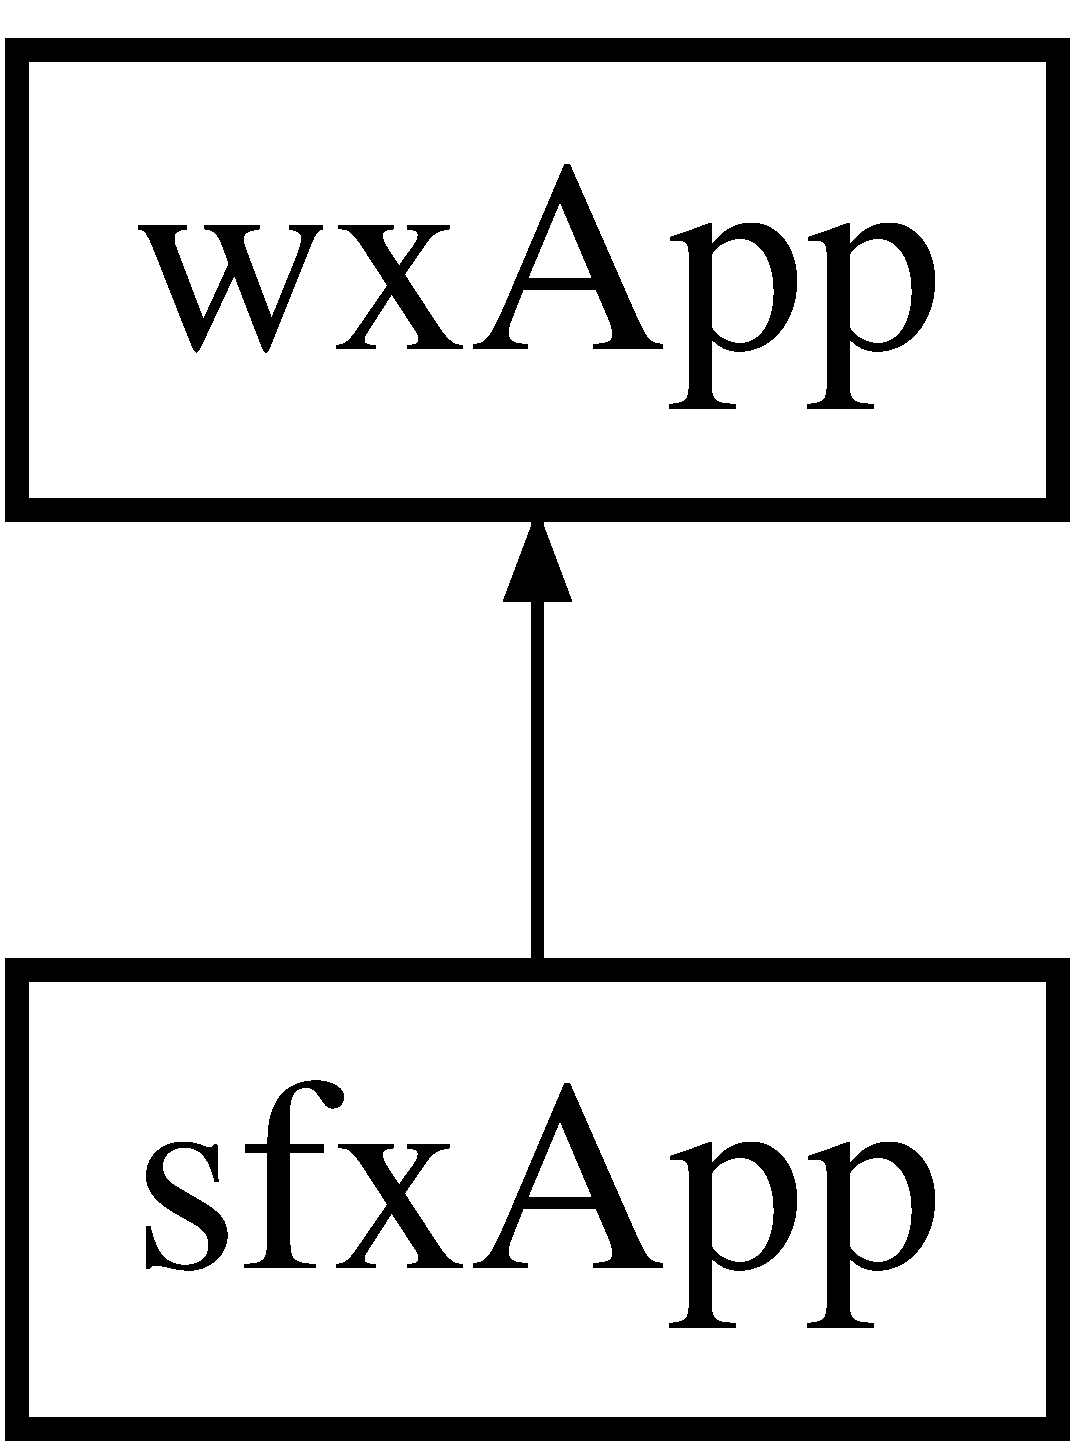
\includegraphics[height=2.000000cm]{classsfx_app}
\end{center}
\end{figure}
\subsection*{Public Member Functions}
\begin{DoxyCompactItemize}
\item 
virtual bool \hyperlink{classsfx_app_a227d3ad9e2fdb29c7dd7b2204f61577c}{On\-Init} ()
\begin{DoxyCompactList}\small\item\em \hyperlink{classsfx_app_a227d3ad9e2fdb29c7dd7b2204f61577c}{On\-Init()} machine generated code to start application + added support for single instance mutex. \end{DoxyCompactList}\item 
virtual int \hyperlink{classsfx_app_ab037c140aacb6010a5015f0d358e5b92}{On\-Exit} ()
\begin{DoxyCompactList}\small\item\em \hyperlink{classsfx_app_ab037c140aacb6010a5015f0d358e5b92}{On\-Exit()} virtual function override. \end{DoxyCompactList}\end{DoxyCompactItemize}


\subsection{Detailed Description}
Defines Application Class. Machine generated. 

Definition at line 19 of file sfx\-App.\-h.



\subsection{Member Function Documentation}
\hypertarget{classsfx_app_ab037c140aacb6010a5015f0d358e5b92}{\index{sfx\-App@{sfx\-App}!On\-Exit@{On\-Exit}}
\index{On\-Exit@{On\-Exit}!sfxApp@{sfx\-App}}
\subsubsection[{On\-Exit}]{\setlength{\rightskip}{0pt plus 5cm}int sfx\-App\-::\-On\-Exit (
\begin{DoxyParamCaption}
{}
\end{DoxyParamCaption}
)\hspace{0.3cm}{\ttfamily [virtual]}}}\label{classsfx_app_ab037c140aacb6010a5015f0d358e5b92}


\hyperlink{classsfx_app_ab037c140aacb6010a5015f0d358e5b92}{On\-Exit()} virtual function override. 

\begin{DoxyReturn}{Returns}
Returns 0 at all times. 
\end{DoxyReturn}


Definition at line 51 of file sfx\-App.\-cpp.

\hypertarget{classsfx_app_a227d3ad9e2fdb29c7dd7b2204f61577c}{\index{sfx\-App@{sfx\-App}!On\-Init@{On\-Init}}
\index{On\-Init@{On\-Init}!sfxApp@{sfx\-App}}
\subsubsection[{On\-Init}]{\setlength{\rightskip}{0pt plus 5cm}bool sfx\-App\-::\-On\-Init (
\begin{DoxyParamCaption}
{}
\end{DoxyParamCaption}
)\hspace{0.3cm}{\ttfamily [virtual]}}}\label{classsfx_app_a227d3ad9e2fdb29c7dd7b2204f61577c}


\hyperlink{classsfx_app_a227d3ad9e2fdb29c7dd7b2204f61577c}{On\-Init()} machine generated code to start application + added support for single instance mutex. 

Guarantee to run only one instance.

\begin{DoxyReturn}{Returns}
false if already running, else wxs\-O\-K. 
\end{DoxyReturn}
Guarantee to run only one instance of this application at all times. Supplied string is a U\-U\-I\-D. 

Definition at line 66 of file sfx\-App.\-cpp.



The documentation for this class was generated from the following files\-:\begin{DoxyCompactItemize}
\item 
sfx/sfx\-App.\-h\item 
sfx/sfx\-App.\-cpp\end{DoxyCompactItemize}

\hypertarget{classsfx_frame}{\section{sfx\-Frame Class Reference}
\label{classsfx_frame}\index{sfx\-Frame@{sfx\-Frame}}
}
Inheritance diagram for sfx\-Frame\-:\begin{figure}[H]
\begin{center}
\leavevmode
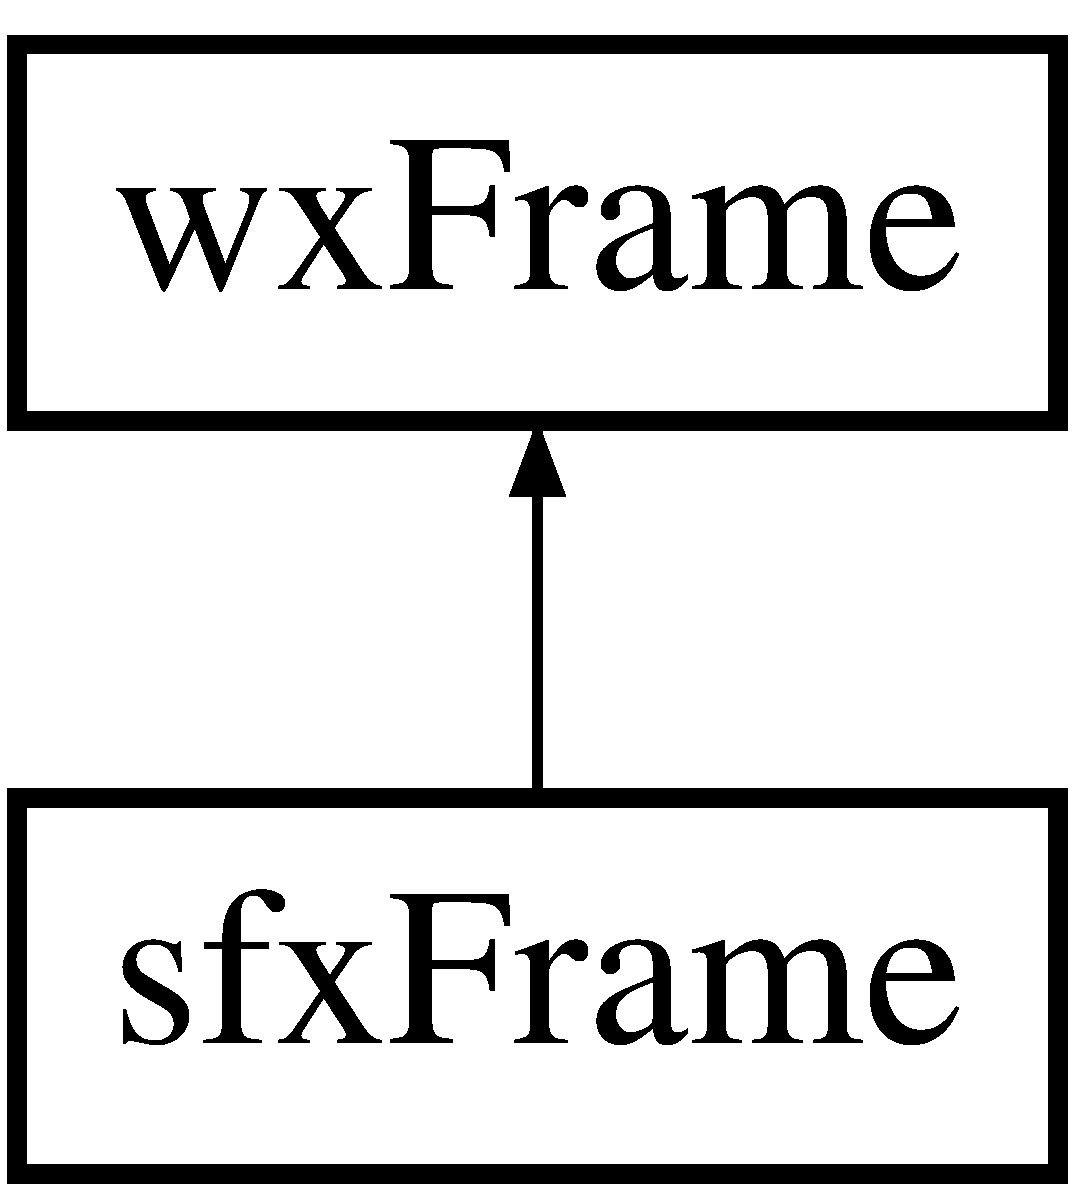
\includegraphics[height=2.000000cm]{classsfx_frame}
\end{center}
\end{figure}
\subsection*{Public Member Functions}
\begin{DoxyCompactItemize}
\item 
\hypertarget{classsfx_frame_a7a333991300687c3d7c47f8dce9c697c}{{\bfseries sfx\-Frame} (wx\-Window $\ast$parent, wx\-Window\-I\-D id=-\/1)}\label{classsfx_frame_a7a333991300687c3d7c47f8dce9c697c}

\end{DoxyCompactItemize}


\subsection{Detailed Description}


Definition at line 30 of file sfx\-Main.\-h.



The documentation for this class was generated from the following files\-:\begin{DoxyCompactItemize}
\item 
sfx/sfx\-Main.\-h\item 
sfx/sfx\-Main.\-cpp\end{DoxyCompactItemize}

\hypertarget{class_utility}{\section{Utility Class Reference}
\label{class_utility}\index{Utility@{Utility}}
}
\subsection*{Static Public Member Functions}
\begin{DoxyCompactItemize}
\item 
static wx\-String \hyperlink{class_utility_a1e1ef24f6c7c1de1e8e5bf8a2c07b278}{include\-Trailing\-Backslash} (const wx\-String folder)
\begin{DoxyCompactList}\small\item\em Ensure a folder ends with a backslash. \end{DoxyCompactList}\item 
static wx\-String \hyperlink{class_utility_a711454ada421834a0d0078e8770ea231}{valid\-File\-Name} (const wx\-String description)
\begin{DoxyCompactList}\small\item\em Turn description into a valid Windows filename. \end{DoxyCompactList}\end{DoxyCompactItemize}


\subsection{Detailed Description}


Definition at line 25 of file utility.\-h.



\subsection{Member Function Documentation}
\hypertarget{class_utility_a1e1ef24f6c7c1de1e8e5bf8a2c07b278}{\index{Utility@{Utility}!include\-Trailing\-Backslash@{include\-Trailing\-Backslash}}
\index{include\-Trailing\-Backslash@{include\-Trailing\-Backslash}!Utility@{Utility}}
\subsubsection[{include\-Trailing\-Backslash}]{\setlength{\rightskip}{0pt plus 5cm}wx\-String Utility\-::include\-Trailing\-Backslash (
\begin{DoxyParamCaption}
\item[{const wx\-String}]{folder}
\end{DoxyParamCaption}
)\hspace{0.3cm}{\ttfamily [static]}}}\label{class_utility_a1e1ef24f6c7c1de1e8e5bf8a2c07b278}


Ensure a folder ends with a backslash. 


\begin{DoxyParams}{Parameters}
{\em folder} & Input folder with or without trailing backslash. \\
\hline
\end{DoxyParams}
\begin{DoxyReturn}{Returns}
wx\-String of folder with a trailing backslash. 
\end{DoxyReturn}


Definition at line 24 of file utility.\-cpp.

\hypertarget{class_utility_a711454ada421834a0d0078e8770ea231}{\index{Utility@{Utility}!valid\-File\-Name@{valid\-File\-Name}}
\index{valid\-File\-Name@{valid\-File\-Name}!Utility@{Utility}}
\subsubsection[{valid\-File\-Name}]{\setlength{\rightskip}{0pt plus 5cm}wx\-String Utility\-::valid\-File\-Name (
\begin{DoxyParamCaption}
\item[{const wx\-String}]{description}
\end{DoxyParamCaption}
)\hspace{0.3cm}{\ttfamily [static]}}}\label{class_utility_a711454ada421834a0d0078e8770ea231}


Turn description into a valid Windows filename. 


\begin{DoxyParams}{Parameters}
{\em description} & Input to turn into a filename \\
\hline
\end{DoxyParams}
\begin{DoxyReturn}{Returns}
Description in such a form that it can be used as a filename under Windows O\-S.
\end{DoxyReturn}
We take a bit of a sharp turn, because we disallow everything but chars, numbers and spaces. And use a max 128 char filename (M\-A\-X\-\_\-\-P\-A\-T\-H in Win32 is longer). 

Definition at line 52 of file utility.\-cpp.



The documentation for this class was generated from the following files\-:\begin{DoxyCompactItemize}
\item 
sfx/utility.\-h\item 
sfx/utility.\-cpp\end{DoxyCompactItemize}

%--- End generated contents ---

% Index
\newpage
\phantomsection
\addcontentsline{toc}{part}{Index}
\printindex

\end{document}
